\documentclass{uLatex}
\usepackage{cleveref}
\usepackage{Ufont}
\usepackage{Ugraphic}

\author{Submission number: 50}
\title{Repeatability Evaluation Package}
\subtitle{HSCC 2021}


\begin{document}
\maketitle[standard]

\section{Requirements}

Following the Repeatability Evaluation guidelines\cite{hscc2021-rer}, we packaged the software and data component inside a Docker Image. The main system requirement to replicate our results is naturally to have Docker installed\cite{get-docker} on your Operating System. We tested with version~19 but any decently recent version should work. Additionally, you will need a Web Browser to interact with the Jupyter Notebooks\cite{jupyter-notebook} included in the image (internet connection is not required). Again, we tested with Google Chrome\cite{google-chrome}, but other standard browsers should work as well.

\section{Download and Install}

Please visit \url{https://uber.box.com/v/hscc-2021-rep-50-v2} and hit the Download button so that you can save \FileName{hscc\_2021\_rep\_50\_notebook\_v2.tar.gz} on your computer. The SHA-256 checksum of this file  is \verb|22196e3f9ab2b538662eff73e3ca5a88c119e2d0d73f1fcc095bef8914dc317b| as computed by \cmdbox*{sha256sum} on Unix-like systems.

\smallskip
Finally, import the image from the downloaded archive in your local registry with:
\begin{bashshell}
docker load < hscc_2021_rep_50_notebook_v2.tar.gz
\end{bashshell}

The image named \FileName{hscc\_2021/rep/50/notebook:v2} should now be available (you can check with \cmdbox{docker image ls})

\section{Run the Software}

Now you can use docker run\cite{docker-run} to start the Jupyter Notebooks:
\begin{bashshell}
docker run --publish 8888:8888 hscc_2021/rep/50/notebook:v2
\end{bashshell}
Follow the link indicated in the standard output to land on the page depicted in \cref{fig:jupyter}:
\begin{figure}[h!]
    \centering
    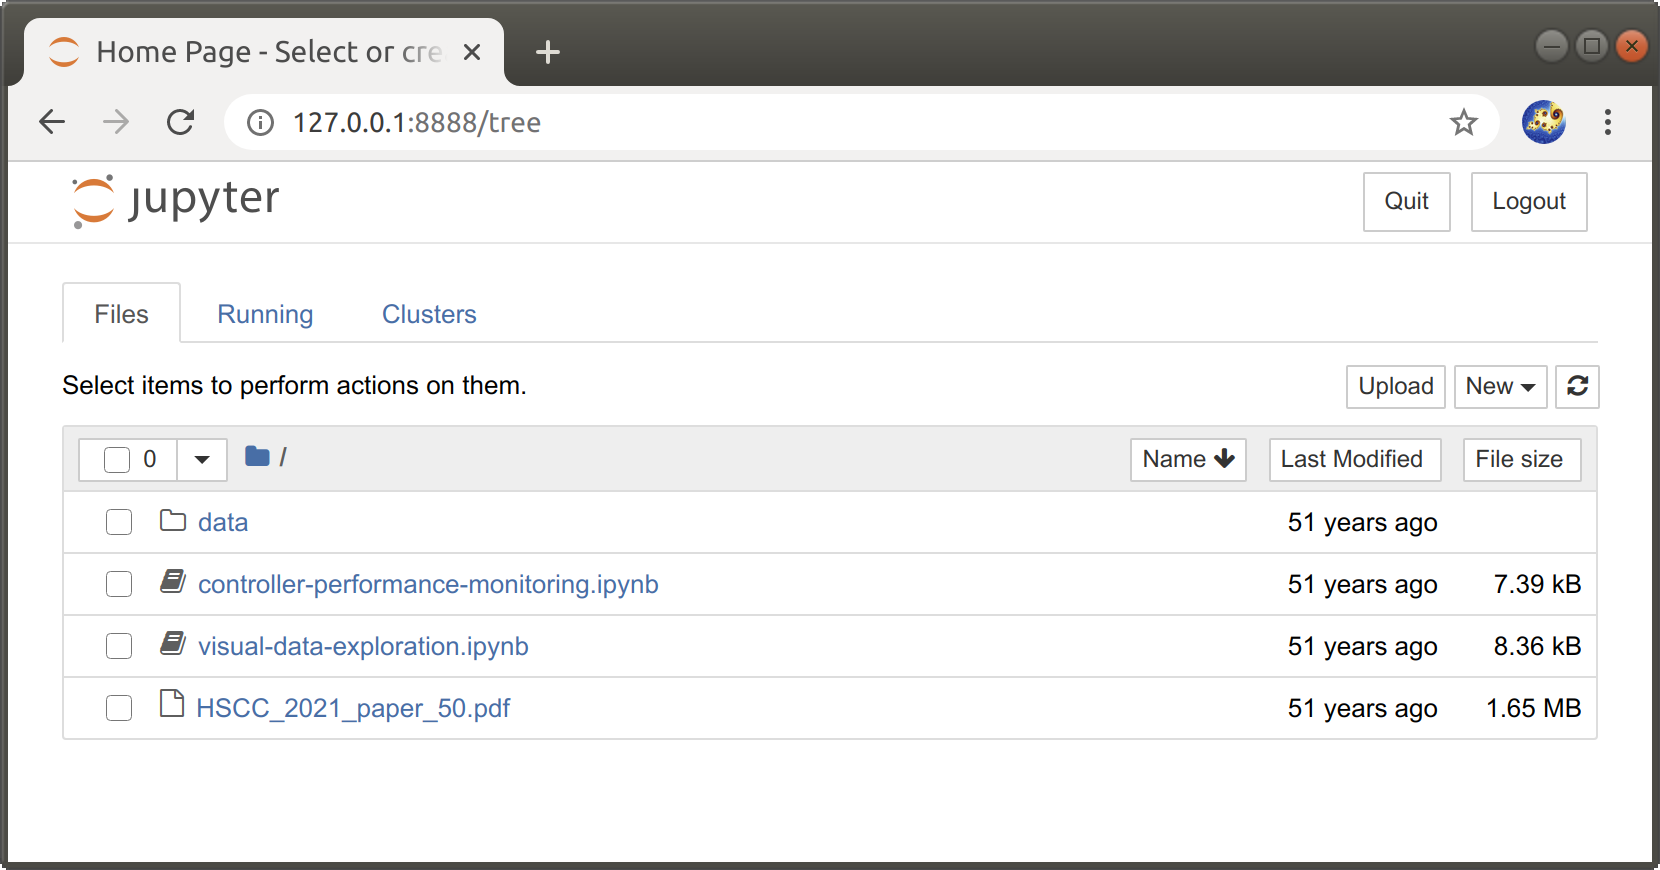
\includegraphics[width=\textwidth]{jupyter}
    \caption{Jupyter Home Page}
    \label{fig:jupyter}
\end{figure}

\section{Content}

The root folder contains a copy of the submitted paper, a \FileName{data} directory with all the inputs required to reproduce our results (or the intermediate results if those are too computational expensive) and two notebooks:
\begin{description}
\item[controller-performance-monitoring.ipynb] This notebook contains the STL evaluation and performance metrics evaluation.
\item[visual-data-exploration.ipynb] This notebook contains the rest of the process, ie visual data exploration,
data extraction and formatting for the paper.
\end{description}

Please visit the respective notebooks by clicking on the filename, you will find there additional documentation on how to replicate our results (\cref{fig:notebooks}).

\begin{figure}[h!]
    \centering\noindent
    \begin{subfigure}[t]{.49\linewidth}
        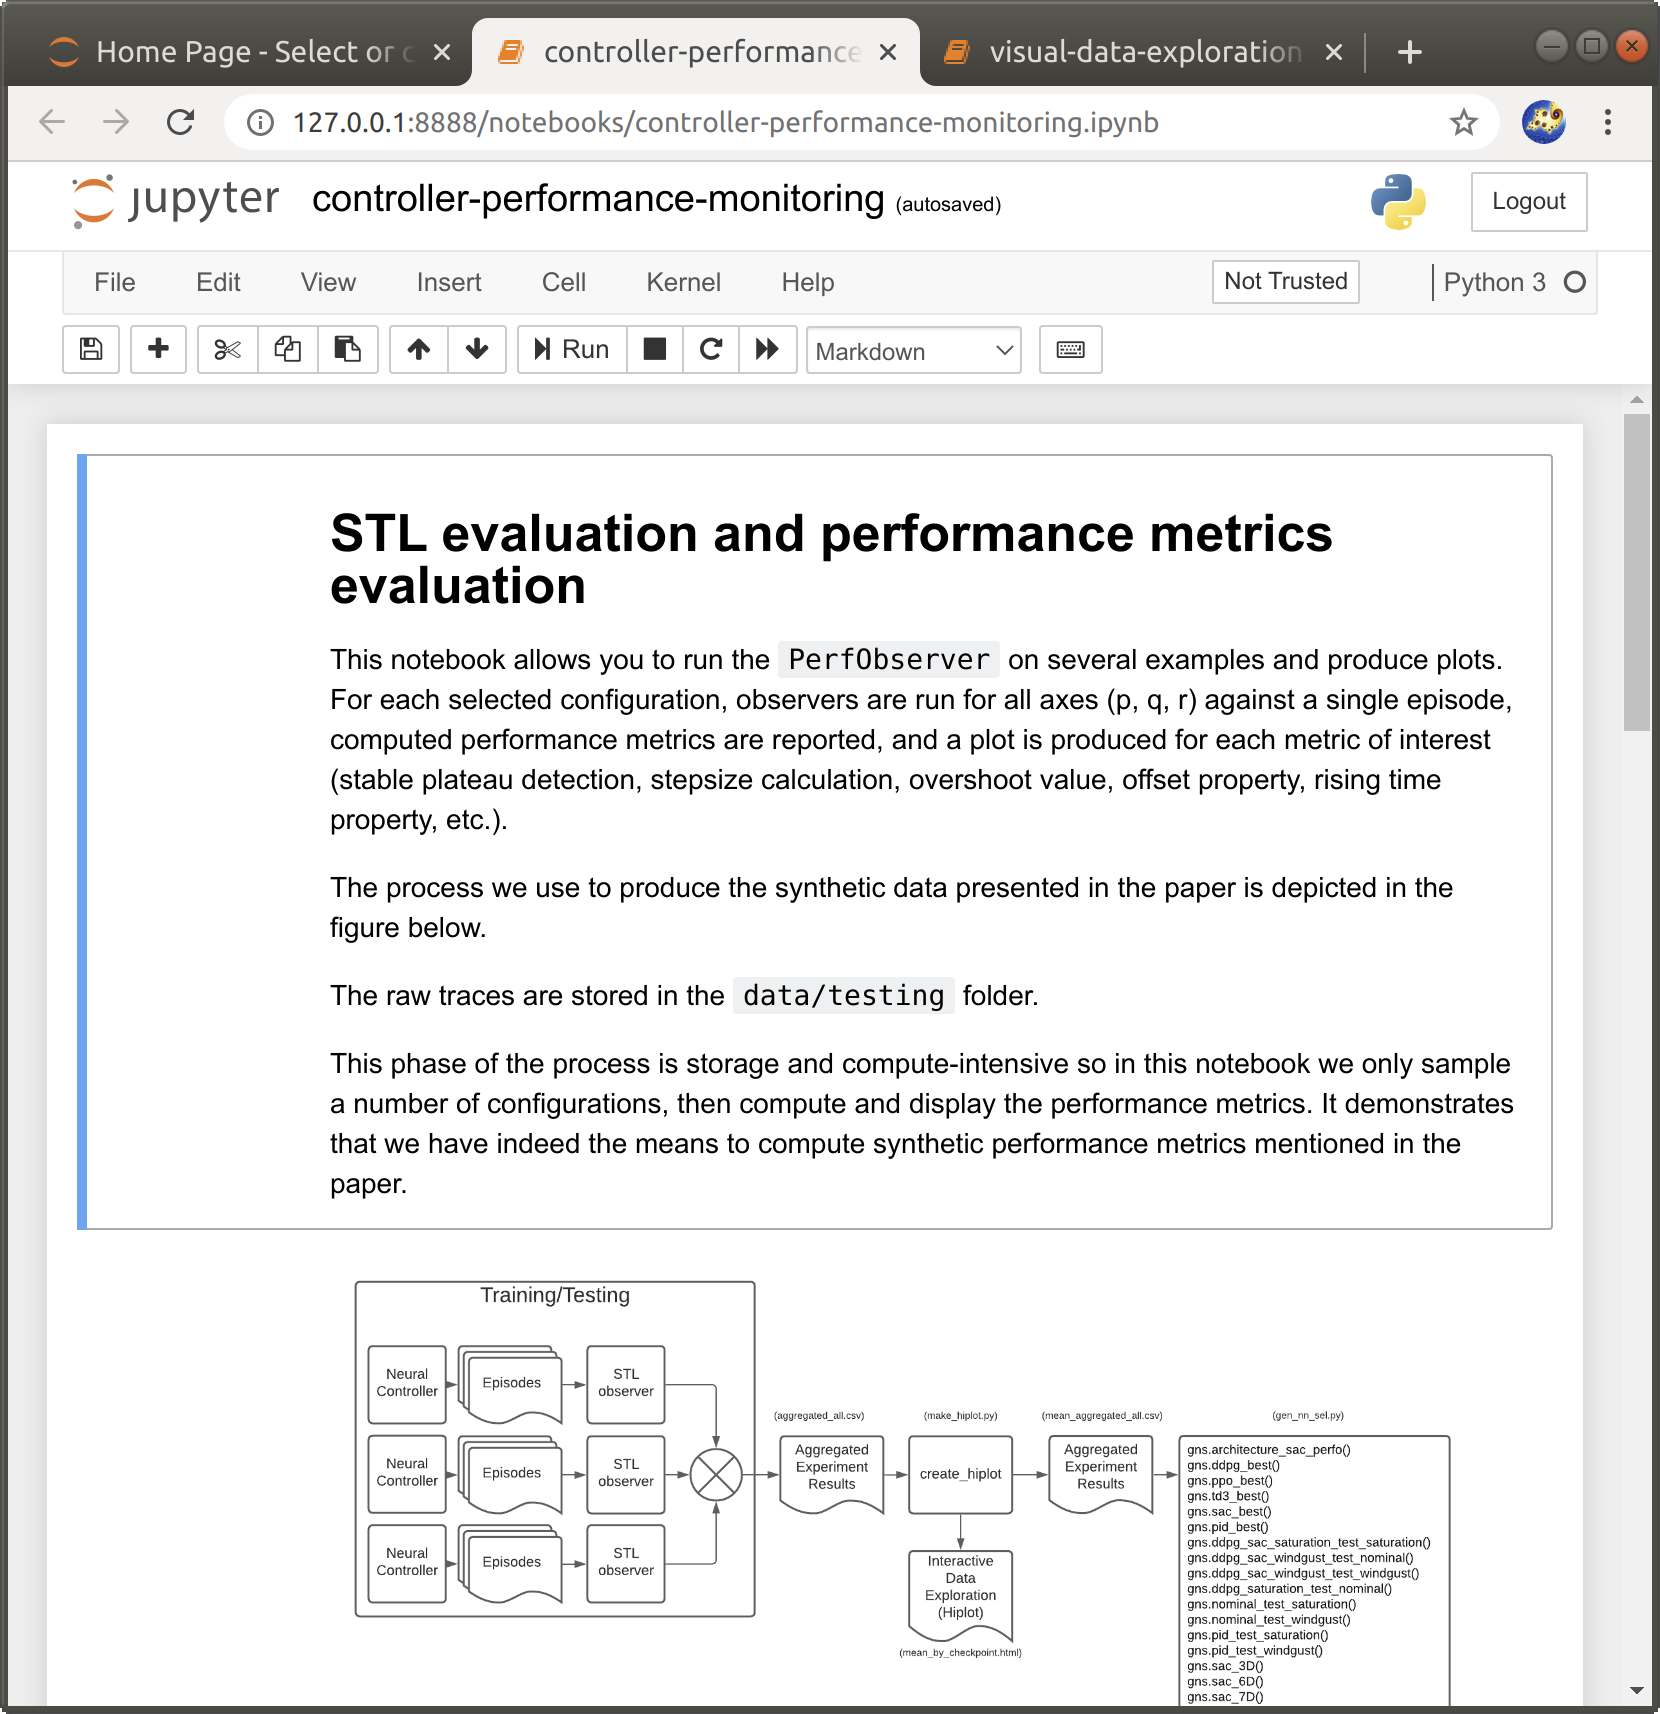
\includegraphics[width=\linewidth]{notebook-1}
        \caption{STL and performance metrics evaluation}
    \end{subfigure}
    \hfill
    \begin{subfigure}[t]{.49\linewidth}
        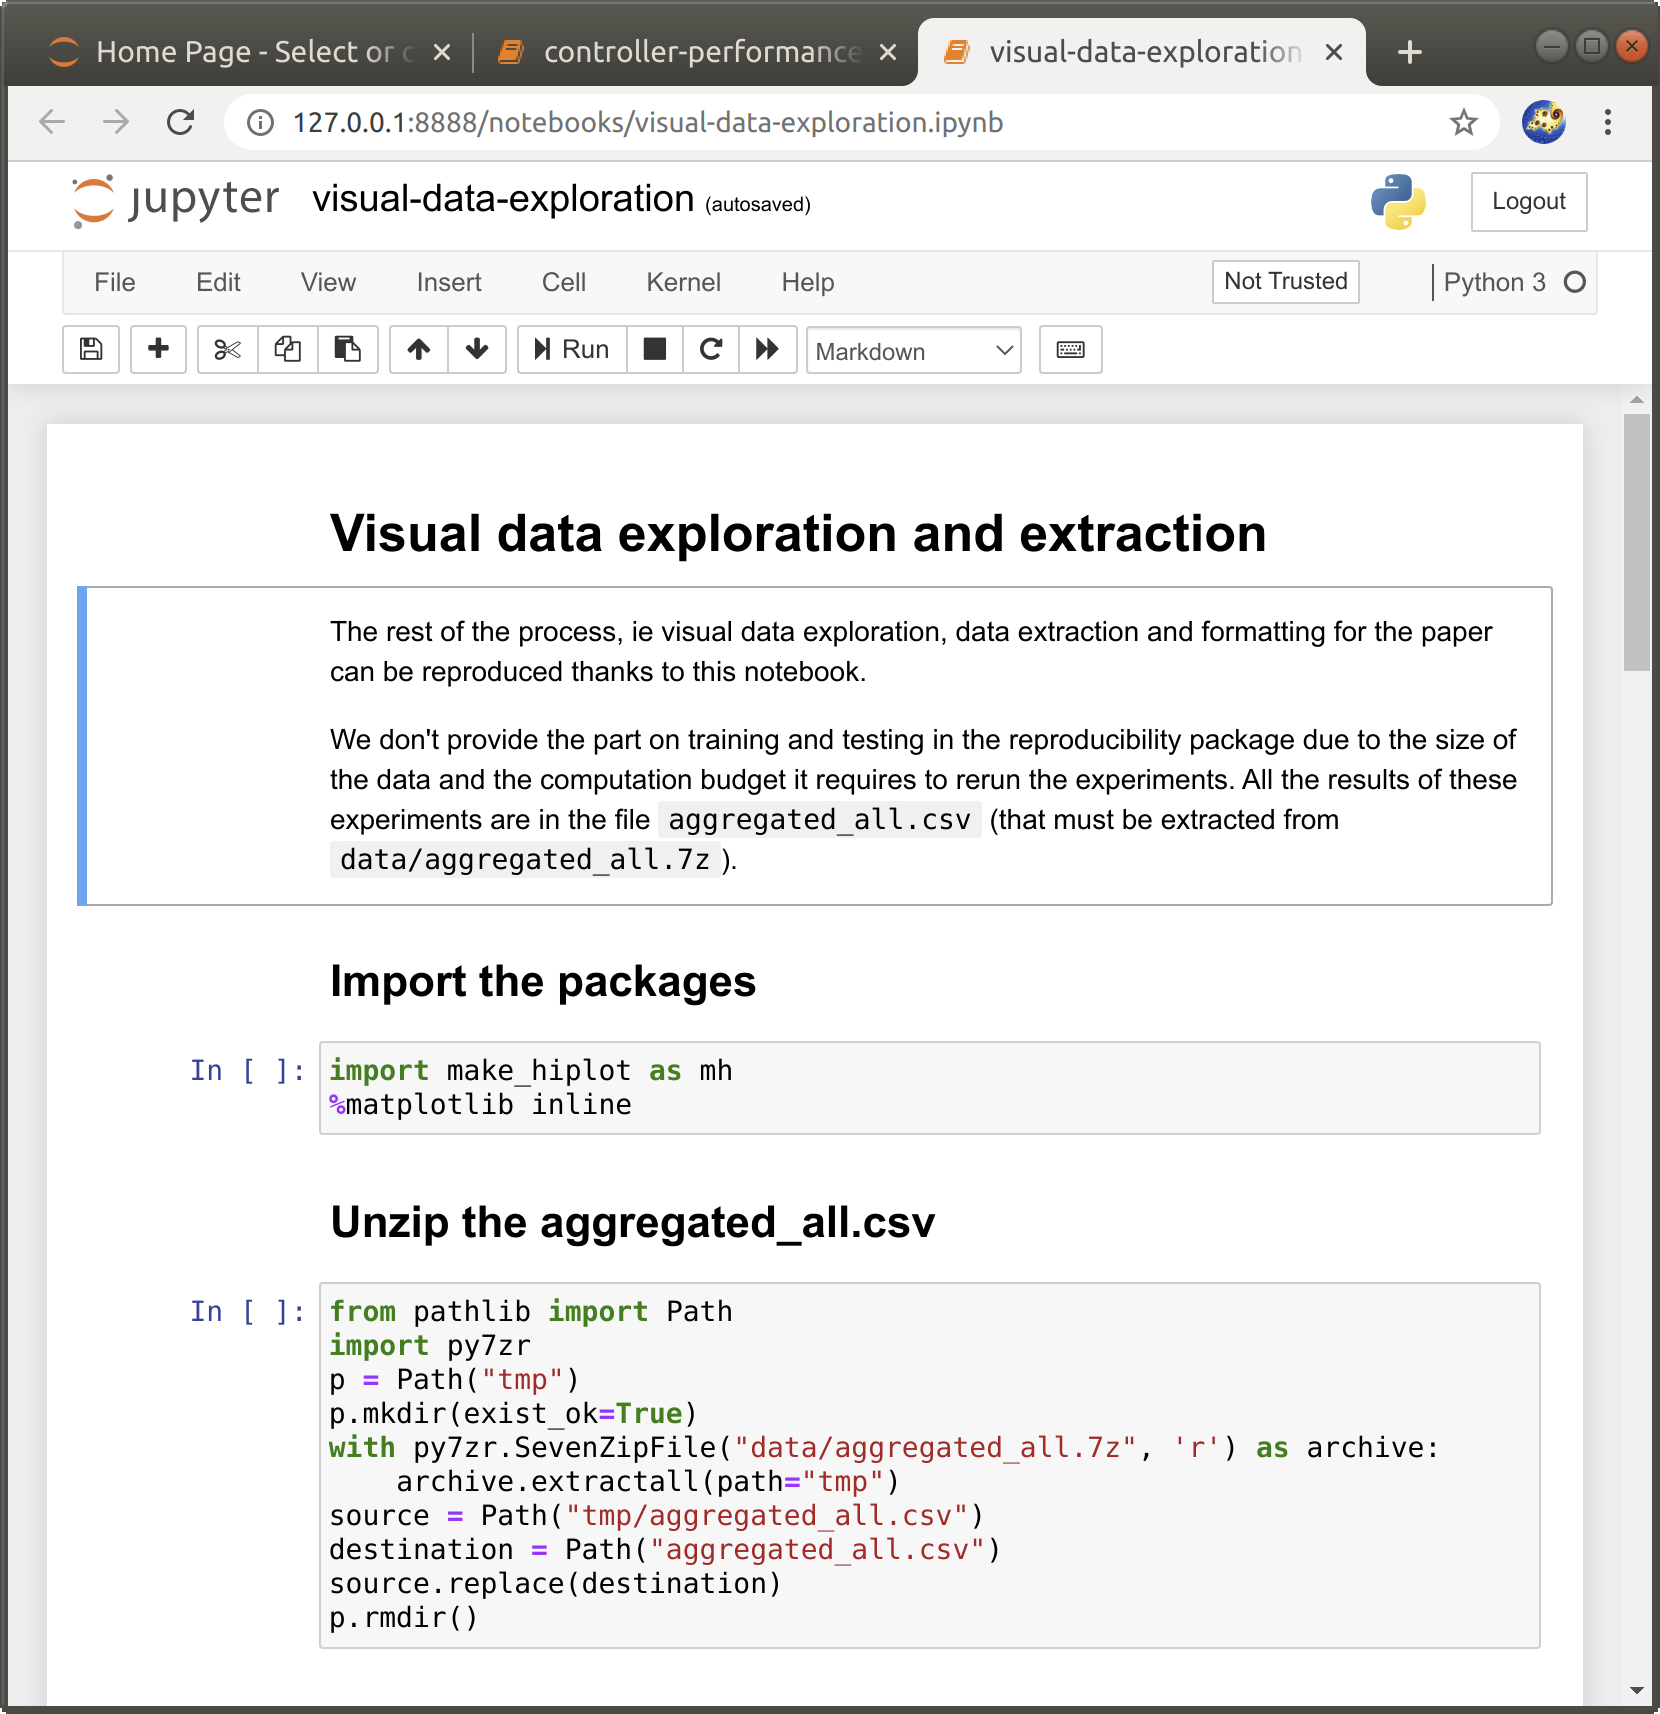
\includegraphics[width=\linewidth]{notebook-2}
        \caption{Visual data exploration and extraction}
    \end{subfigure}
    \caption{Jupyter Notebooks}
    \label{fig:notebooks}
\end{figure}

\printbibliography
\end{document}
